\documentclass{article}
\usepackage{graphicx}
\usepackage{amsmath}
\usepackage{amssymb}
\usepackage{hyperref}
\usepackage{float}
\usepackage{tikz}
\usepackage{subcaption} % for subfigures
\usepackage{listings}
\usetikzlibrary{arrows.meta,calc,positioning}

\title{CSC420 Assignment 3}
\author{Zixuan Zeng 1008533419}

\begin{document}
\date{}
\maketitle
% \raggedright
% (Note: The notebook has been rerun, results could be different from the report.)\newline


\newpage
\section*{Part I: Theoretical Problems}
\subsection*{Question 1: RANSAC}
\subsubsection*{1.1}
Based on description, we have:\newline
$
\begin{aligned}
    p &= 99.5\% = 0.995\\
    (1 - e) &= 70\% = 0.7\\
    s &= 4\\
\end{aligned}
$\newline
The number of iterations(samples) to fit the homography:\newline
$
\begin{aligned}
    N &= \frac{log(1-p)}{log(1-(1-e)^s)}\\
    &=\frac{log(1-0.995)}{log(1-0.7^4)}\\
    &=\frac{log(0.005)}{log(0.7599)}\\
    &=\frac{-2.30102999566}{-0.11924355549}\\
    &\approx 19.2969
\end{aligned}
$\newline
Therefore, we need $\lceil N \rceil = \lceil 19.2969 \rceil = 20$ iterations to fit the homography.

\subsubsection*{1.2}
Affine transformation requires 3 pairs of corresponding points, instead of 4 pairs.
With a smaller s, the probability of having an all-inlier sample increases. Therefore N decreses, fewer RANSAC iterations are needed.


\newpage
\subsection*{Question 2: Camera Models}
\subsubsection*{2.1}
Pixel coordinates of the line in the image:\newline
$
\begin{aligned}
    \vec{p} &= 
    \begin{bmatrix}
        wx\\
        wy\\
        w
    \end{bmatrix}
    = K\vec{P}\\
    &=
    \begin{bmatrix}
        f & 0 & p_x\\
        0 & f & p_y\\
        0 & 0 & 1
    \end{bmatrix}
    \cdot
    \begin{bmatrix}
        X_0 + td_x\\
        Y_0 + td_y\\
        Z_0 + td_z
    \end{bmatrix}\\
    &=
    \begin{bmatrix}
        fX_0 + ftd_x + p_x Z_0 + p_x td_z\\
        fY_0 + ftd_y + p_y Z_0 + p_y td_z\\
        Z_0 + td_z
    \end{bmatrix}\\
\end{aligned}
$\newline\newline
Vanishing coordinates of the line:\newline
$
\begin{aligned}
    x &= \lim_{t \rightarrow \infty} 
        \frac{fX_0 + ftd_x + p_x Z_0 + p_x td_z}{Z_0 + td_z}
        = \frac{fd_x + p_x d_z}{d_z} = p_x + \frac{fd_x}{d_z}\\
    y &= \lim_{t \rightarrow \infty} 
        \frac{fY_0 + ftd_y + p_y Z_0 + p_y td_z}{Z_0 + td_z}
        = \frac{fd_y + p_y d_z}{d_z} = p_y + \frac{fd_y}{d_z}\\
\end{aligned}
$\newline\newline
We have the vanishing point for line L at: \newline
$(p_x + \frac{fd_x}{d_z}, p_y + \frac{fd_y}{d_z})$.

\subsubsection*{2.2}
% In part 2.1, I've proven the vanishing point on the image only depends on the direction of the line: $\vec{d} = [d_x,d_y,d_z]$, and not on which points it passes through.\newline
Following hint, since the line lies on the plane, we have:
\[
\vec{n} \cdot \vec{d} = n_x d_x + n_y d_y + n_z d_z = 0.
\]
\[
n_x \frac{d_x}{d_z} + n_y \frac{d_y}{d_z} + n_z = 0,
\]
From Part 1, the vanishing point corresponding to a line with direction \(\vec{d}\) is given by
\[
(x, y) = \left(f\,\frac{d_x}{d_z} + p_x,\; f\,\frac{d_y}{d_z} + p_y\right).
\]
we have:
\[
\frac{d_x}{d_z} = \frac{x - p_x}{f}, \quad \frac{d_y}{d_z} = \frac{y - p_y}{f}.
\]
Substituting these into the condition gives
\[
n_x \frac{x - p_x}{f} + n_y \frac{y - p_y}{f} + n_z = 0.
\]
Multiplying through by \(f\) results in:
\[
n_x (x - p_x) + n_y (y - p_y) + n_z f = 0.
\]
This equation represents a straight line in the image plane. Therefore, the vanishing points of all lines lying on the plane lie on this line horizon. 


\newpage
\subsection*{Question 3: Homogeneous Coordinates}
\subsubsection*{3.1}
Let the homogeneous coordinates of the two lines be:\newline
$
l = \begin{bmatrix} a \\ b \\ c \end{bmatrix}, \quad l' = \begin{bmatrix} a' \\ b' \\ c' \end{bmatrix}.
$\newline
point $p$ via cross product:\newline
$
p = l \times l' 
= \begin{vmatrix}
    i & j & k\\
    a & b & c\\
    a' & b' & c'\\
\end{vmatrix}
=\begin{bmatrix}
    b c' - c b' \\[1mm] 
    c a' - a c' \\[1mm] 
    a b' - b a' 
\end{bmatrix}.
$\newline
To show that \( p \) is the intersection of \( l \) and \( l' \), we need to verify that \( p \) lies on both lines:\newline
$
\begin{aligned}
    l^T p &= a (b c' - c b') + b (c a' - a c') + c (a b' - b a')\\
    &= a b c' - a c b' + b c a' - b a c' + c a b' - c b a'\\
    &= 0
\end{aligned}
$\newline
Similarly:\newline
$
\begin{aligned}
    l'^T p &= a' (b c' - c b') + b' (c a' - a c') + c' (a b' - b a')\\
    &= a' b c' - a' c b' + b' c a' - b' a c' + c' a b' - c' b a'\\
    &= 0
\end{aligned}
$\newline
Since \( p \) satisfies \( l^T p = 0 \) and \( l'^T p = 0 \), it lies on both lines \( l \) and \( l' \). Therefore, the intersection of the two lines in homogeneous coordinates is given by:
$p = l \times l'$.

\subsubsection*{3.2}
Let the homogeneous coordinates of the two points be:\newline
$
p = \begin{bmatrix} x \\ y \\ 1 \end{bmatrix}, 
\quad p' = \begin{bmatrix} x' \\ y' \\ 1 \end{bmatrix}.
$\newline
line $l$ via cross product:\newline
$
l = p \times p' 
= \begin{vmatrix}
    i & j & k\\
    x & y & 1\\
    x' & y' & 1\\
\end{vmatrix}
=\begin{bmatrix}
    y - y' \\[1mm] 
    x' - x \\[1mm] 
    xy' - x'y 
\end{bmatrix}.
$\newline
To show that \( l \) goes through \( p \) and \( p' \):\newline
$
\begin{aligned}
    l^T p &= (y - y') x + (x' - x) y + (xy' - x'y) 1\\
    &= yx - y'x + x'y - xy + xy' - x'y\\
    &= 0
\end{aligned}
$\newline
Similarly:\newline
$
\begin{aligned}
    l^T p' &= (y - y') x' + (x' - x) y' + (xy' - x'y) 1\\
    &= yx' - y'x' + x'y' - xy' + xy' - x'y\\
    &= 0
\end{aligned}
$\newline
Since \( l \) satisfies \( l^T p = 0 \) and \( l^T p' = 0 \), it goes through \( p \) and \( p' \), and satisfies: $l = p \times p'$.



\newpage
\section*{Part II: Implementation Tasks}
\subsection*{Question 4: Homography}
\subsubsection*{4.1 corresponding points}
\begin{figure}[H]
    \centering
    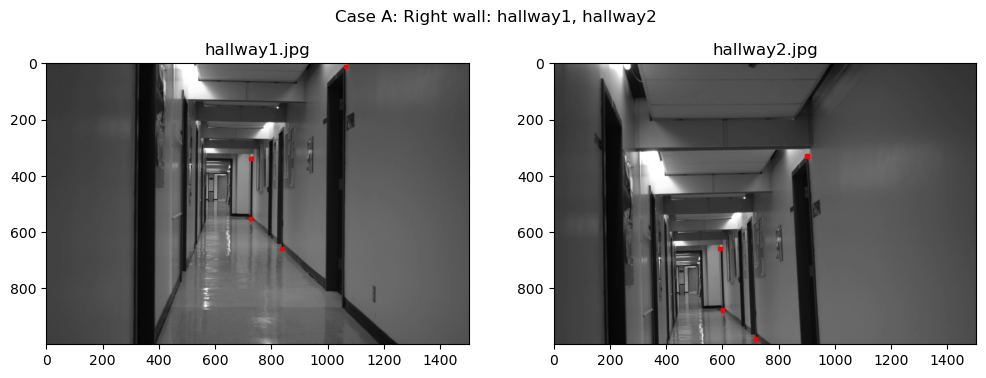
\includegraphics[width=1\textwidth]{4.1.1.png}
\end{figure}
\begin{figure}[H]
    \centering
    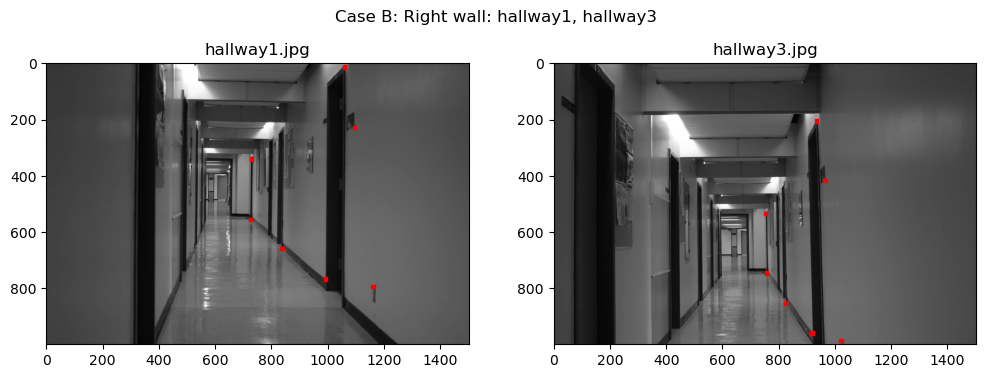
\includegraphics[width=1\textwidth]{4.1.2.png}
\end{figure}
\begin{figure}[H]
    \centering
    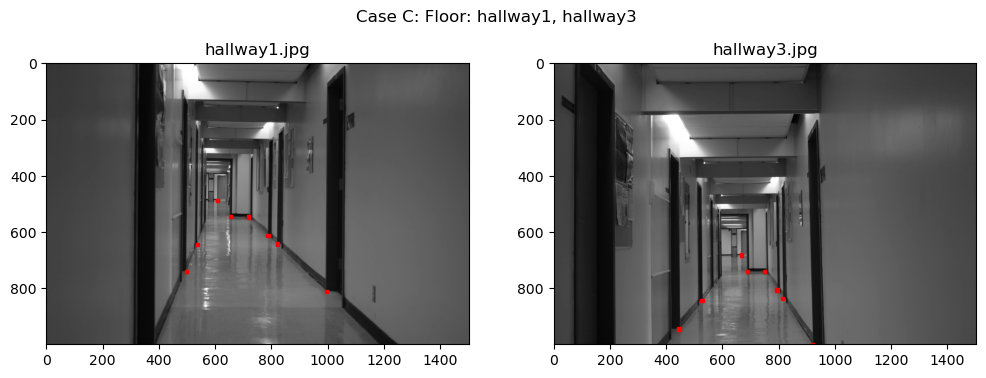
\includegraphics[width=1\textwidth]{4.1.3.png}
\end{figure}

\newpage
\subsubsection*{4.2 fitting homography}
\begin{itemize}
    \item Case A: Right wall: hallway1, hallway2\newline
    Estimated Homography (H) =\newline
    [[ 1.11418672e+00  6.45826835e-03 -1.95425538e+02]\newline
    [ 1.07535227e-02  1.00748626e+00  3.38631466e+02]\newline
    [ 9.21056763e-05 -6.81090744e-05  1.00000000e+00]]\newline
    Scaling: From entries (1,1) and (2,2), approximately 1.114 and 1.007, the image is slightly scaled up both horizontally and vertically.\newline
    Translation: From entries (1,3) and (2,3), the image is shifted x = -195 and y = 339 by large amounts.\newline
    Shear/Rotation: From entries (1,2) and (2,1), (0.00646, 0.01075), there is only a minimal shear (or rotation) effect.
    \item Case B: Right wall: hallway1, hallway3\newline
    Estimated Homography (H) =\newline
    [[ 5.34898952e-01  6.85763306e-03  3.35930226e+02]\newline
    [-3.33510849e-02  9.41727594e-01  2.20856776e+02]\newline
    [-3.25040521e-05 -2.51289448e-05  1.00000000e+00]]\newline
    Scaling: the image is scaled down horizontally by 0.535, and slightly down vertically by 0.942.\newline
    Translation: the image is shifted x = 336 and to y = 221.\newline
    Shear/Rotation: there is only a minimal shear or rotation effect: (0.00686, 0.03335).
    \item Case C: Floor: hallway1, hallway3\newline
    Estimated Homography (H) =\newline
    [[ 1.09817473e+00 -4.38647155e-01  2.32965909e+02]\newline
    [ 4.12180152e-02  1.02463157e+00  1.81945408e+02]\newline
    [ 7.87914388e-05 -2.84615181e-05  1.00000000e+00]]\newline
    Scaling: the image is scaled up horizontally by 1.098, and vertically by 1.025.\newline
    Translation: the image is shifted x = 233 and to y = 182.\newline
    Shear/Rotation: there is significant shear or rotation effect: (-0.438, 0.041), tilted counterclockwise.
\end{itemize}

\newpage
\subsubsection*{4.3 mapping via homography}
Case A: Right wall: hallway1, hallway2:
\begin{figure}[H]
    \centering
    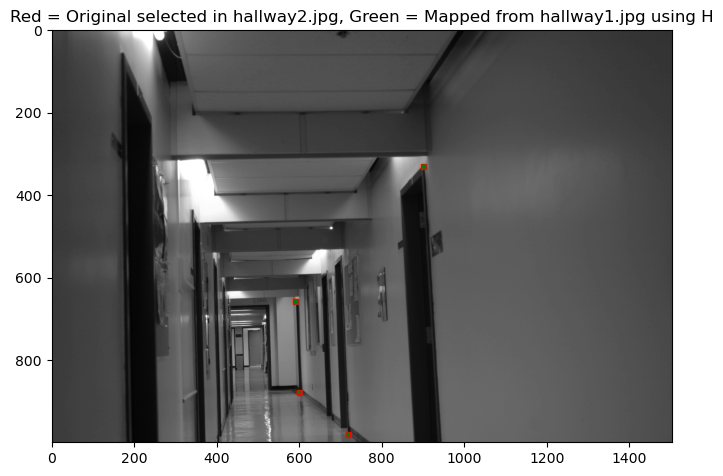
\includegraphics[width=0.6\textwidth]{4.3.1.png}
\end{figure}\noindent
Case B: Right wall: hallway1, hallway3:
\begin{figure}[H]
    \centering
    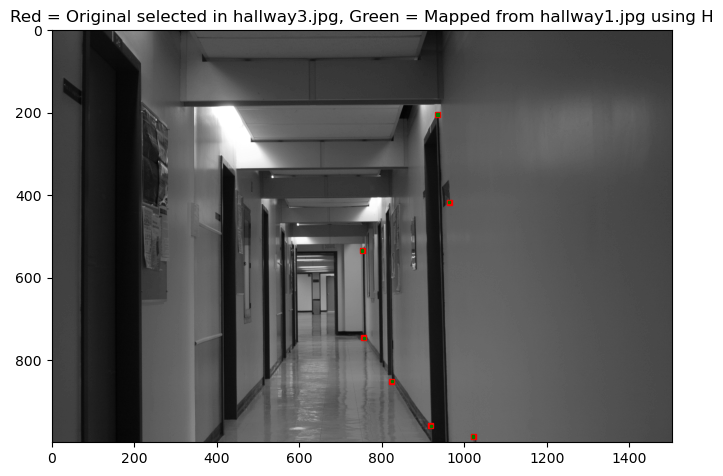
\includegraphics[width=0.6\textwidth]{4.3.2.png}
\end{figure}\noindent
Case C: Floor: hallway1, hallway3:
\begin{figure}[H]
    \centering
    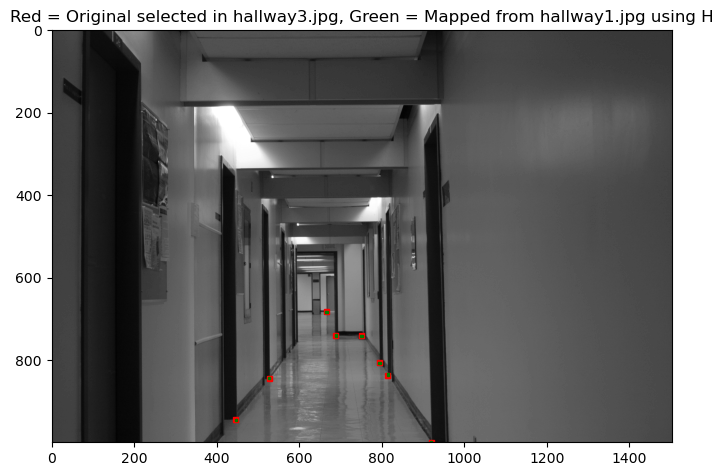
\includegraphics[width=0.6\textwidth]{4.3.3.png}
\end{figure}

\newpage
\subsubsection*{4.4 merged image}
Case A: Right wall: hallway1, hallway2:
\begin{figure}[H]
    \centering
    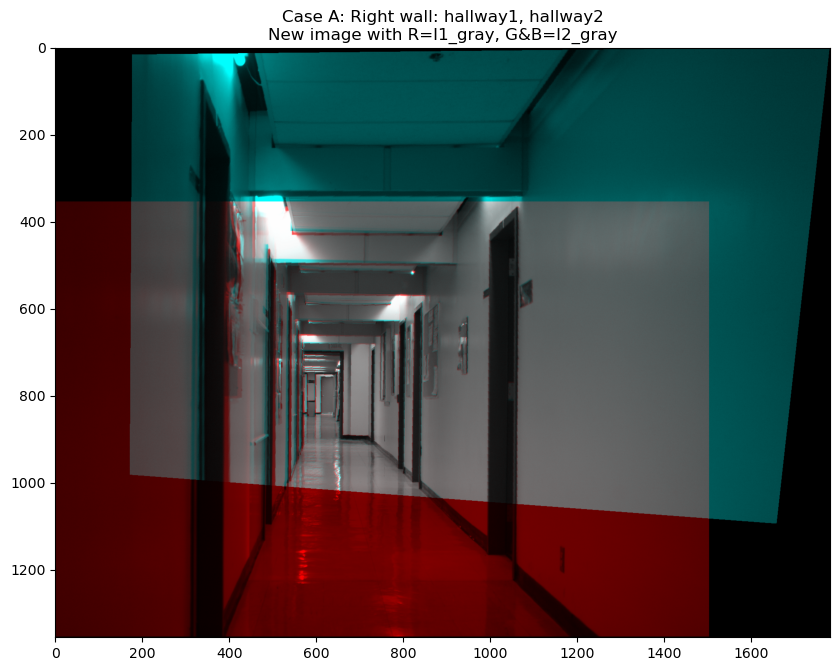
\includegraphics[width=0.6\textwidth]{4.4.1.png}
\end{figure}\noindent
Case B: Right wall: hallway1, hallway3:
\begin{figure}[H]
    \centering
    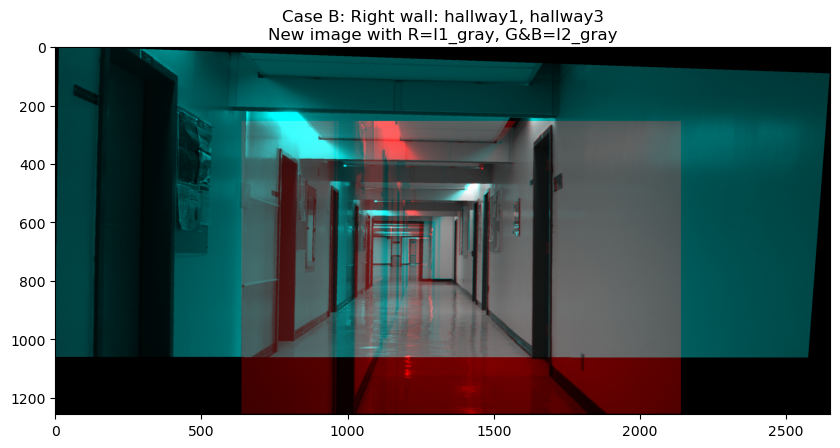
\includegraphics[width=0.6\textwidth]{4.4.2.png}
\end{figure}\noindent
Case C: Floor: hallway1, hallway3:
\begin{figure}[H]
    \centering
    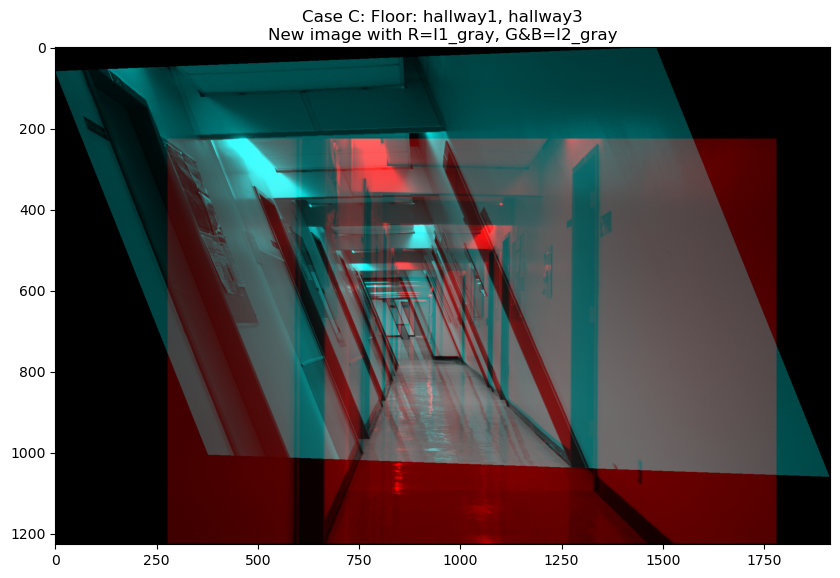
\includegraphics[width=0.6\textwidth]{4.4.3.png}
\end{figure}\noindent
Conclusion:

In Case A, hallway1 and hallway2 have similar 3D position 
but have different orientations, and the merged image show 
very little parallax within the shared region.
However, in Cases B and C, hallway1 and hallway3 have 
very different 3D positions, and the merged image show 
very significant parallax. Therefore, parallax is dependent 
on the position of the camera instead of the viewing angle.

The right wall in Cases A and B shows a consistent gray 
in the shared regions, suggesting it is close to Lambertian. 
The floor in Case C, however, shows more variation, 
and therefore is less Lambertian.

% \newpage
\subsubsection*{4.5 Switch cases code}
\begin{lstlisting}
# Change to 'B' or 'C' as needed
# rerun entire Question 4 after change
case = 'A'  

if case == 'A':
    case_description = "Right wall: hallway1, hallway2"
    img1_path = 'hallway1.jpg'  # I1
    img2_path = 'hallway2.jpg'  # I2
    pts1 = np.array([[727.17975096, 337.84330464],
                    [1062.7991877, 11.95196751],
                    [837.10727662, 659.84340192],
                    [726.206941, 552.83430614]], dtype=float)
    pts2 = np.array([[590.98635634, 657.89778199],
                    [901.31273408, 330.06082494],
                    [718.42446131, 980.87068924],
                    [599.74164599, 877.75283331]], dtype=float)
elif case == 'B':
    case_description = "Right wall: hallway1, hallway3"
    img1_path = 'hallway1.jpg'
    img2_path = 'hallway3.jpg'
    pts1 = np.array([[729.12537088, 340.76173452],
                    [1059.88075782, 12.92477747],
                    [1095.8747264, 228.88858894],
                    [1161.05299382, 793.11836665],
                    [992.75687047, 767.82530765],
                    [838.08008658, 658.87059195],
                    [726.206941, 554.77992607]], dtype=float)
    pts2 = np.array([[753.44561992, 534.35091687],
                    [934.38827278, 204.5683399],
                    [964.54538158, 417.61372148],
                    [1021.94116932, 985.73473904],
                    [918.82331339, 959.46887008],
                    [824.46074712, 852.45977431],
                    [756.36404981, 746.4234885]], dtype=float)
elif case == 'C':
    case_description = "Floor: hallway1, hallway3"
    img1_path = 'hallway1.jpg'
    img2_path = 'hallway3.jpg'
    pts1 = np.array([[609.46974561, 487.65603872],
                    [655.1918138, 545.05182645],
                    [718.42446131, 546.99744637],
                    [788.46677854, 613.14852376],
                    [821.54231723, 642.33282261],
                    [995.67530036, 812.57456588],
                    [497.59660003, 741.55943869],
                    [536.50899849, 644.27844253]], dtype=float)
    pts2 = np.array([[666.86553334, 682.21803103],
                    [688.2673525, 740.58662873],
                    [750.52719004, 741.55943869],
                    [794.30363831, 806.73770611],
                    [814.7326475, 836.89481492],
                    [919.79612335, 999.35407851],
                    [446.03767207, 944.87672066],
                    [526.78089888, 844.67729462]], dtype=float)
\end{lstlisting}


\newpage
\subsection*{Question 5: Mean Shift Tracking}
\subsubsection*{5.1 Performance Evaluation}
IoU over time:
\begin{figure}[H]
    \centering
    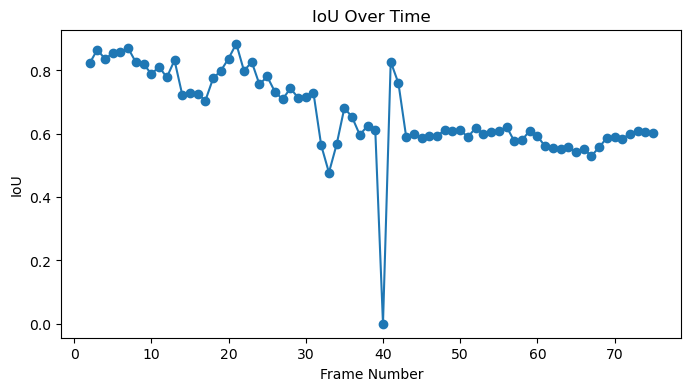
\includegraphics[width=0.6\textwidth]{5.1.1.png}
\end{figure}\noindent
Sample frames:\newline
High IoU: $88.45\% > 50\%$\newline
Low IoU: $0\% < 10\%$, where Viola-Jones failed to detect the face.
\begin{figure}[H]
    \centering
    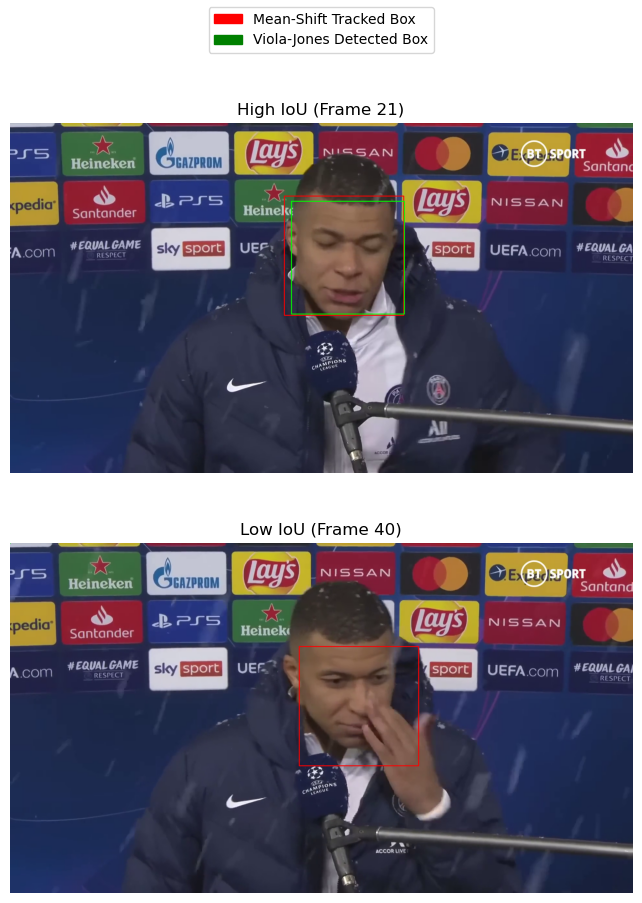
\includegraphics[width=0.6\textwidth]{5.1.2.png}
\end{figure}\noindent
The percentage of frames in which the IoU is larger than 50\%: 97.30\%.

In the frame where the IoU is below 10\%, the Mean-Shift tracked 
bounding box appears to be correct more often than the 
Viola-Jones detection. This is likely because Viola-Jones 
fails when the face is partially blocked or changes orientation, 
while the Mean-Shift tracker remains locked onto the 
color distribution it learned from the initial frame.

\newpage
\subsubsection*{5.2 Implement a Simple Variation}
IoU over time:
\begin{figure}[H]
    \centering
    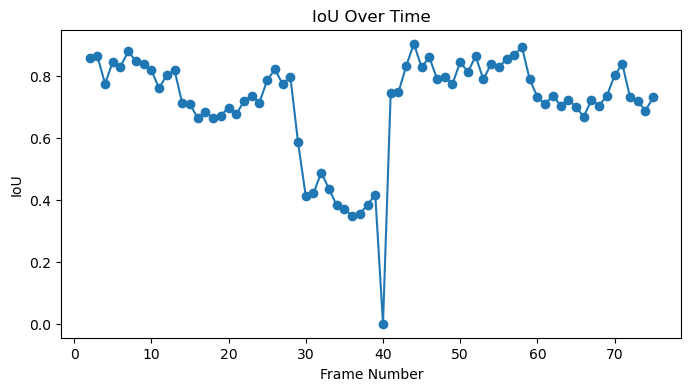
\includegraphics[width=0.6\textwidth]{5.2.1.png}
\end{figure}\noindent
Sample frames:\newline
High IoU: $90.48\% > 80\%$\newline
Low IoU: $38.42\% < 50\%$.
It's worth noting that the lowest IoU is still 0\%, where Viola-Jones failed to detect the face. 
Here, I picked another non-zero low IoU.
\begin{figure}[H]
    \centering
    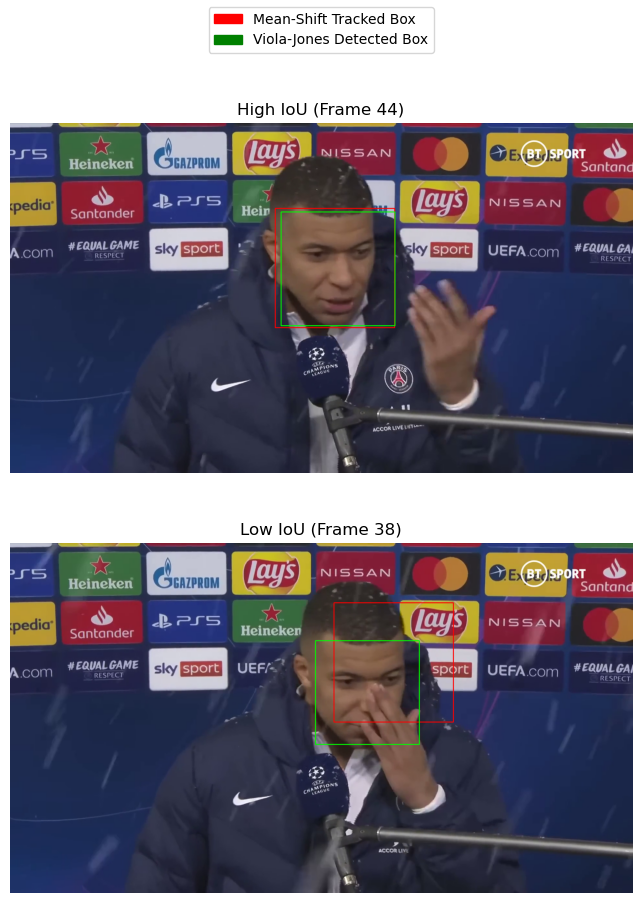
\includegraphics[width=0.6\textwidth]{5.2.2.png}
\end{figure}\noindent
The percentage of frames in which the IoU is larger than 50\%: 85.14\%.










\end{document}

% \begin{figure}[H]
%   \centering
%   \includegraphics[width=0.48\textwidth]{IV.c.png}
%   \caption{ResNeXt32 Test Accuracy: DBI vs SDD}
% \end{figure}

% \begin{figure}[H]
%     \begin{minipage}{0.5\textwidth}
%         \centering
%         \includegraphics[width=\textwidth]{3.1.1.1.png}
%         \caption{image1.png}
%     \end{minipage}
%     \hfill
%     \begin{minipage}{0.5\textwidth}
%         \centering
%         \includegraphics[width=\textwidth]{3.1.2.1.png}
%         \caption{image2.png}
%     \end{minipage}
% \end{figure}